\label{sec:risk-assessment}
The following tables identify various risks and hazards associated with the use of our aircraft, following a standard University of Melbourne Risk Assessment template, shown in Figure \ref{fig:risk-matrix}.\\

Each row of the risk assessment tables contains the following information: the potential hazard, the likelihood of that hazard occurring during the mission, a ``rating'' of the consequence of that hazard, and an assessment of the overall risk for that hazard. Management and mitigation of these risks will be discussed in Section \ref{sec:risk-management}.

\begin{figure}[H]
	
	\begin{subfigure}{\linewidth}
		\centerline{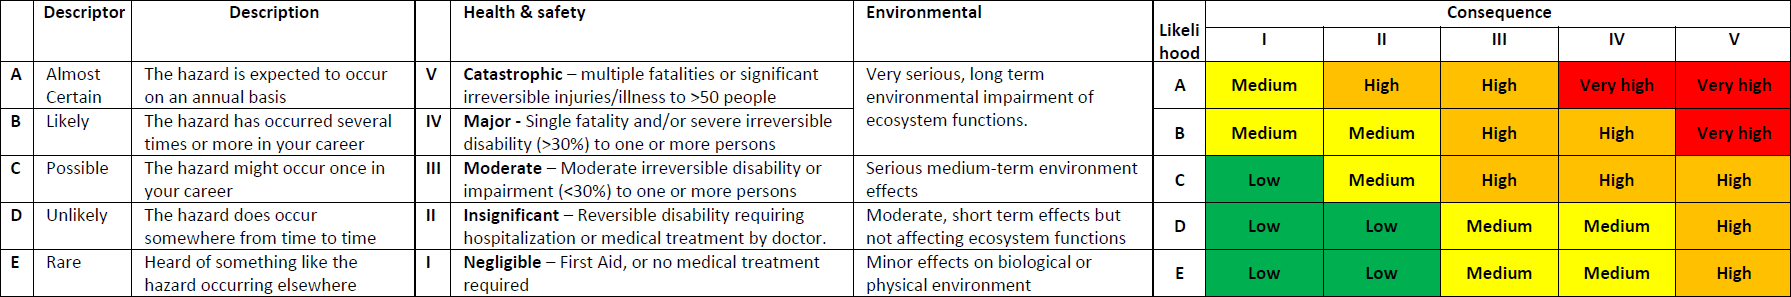
\includegraphics[width=550pt]{../Images/risk-matrix}}
	\end{subfigure}\\[2ex]
	
	\begin{subfigure}{\linewidth}
		\centerline{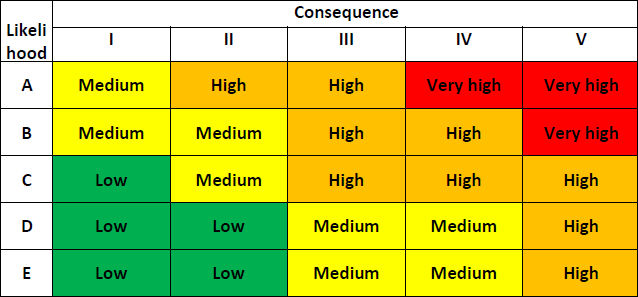
\includegraphics[width=300pt]{../Images/risk-matrix-2}}
	\end{subfigure}
	
	\caption{Risk Management Matrix}
	\label{fig:risk-matrix}
\end{figure}

\begin{table}[!ht]
	\label{tab:risks-electrical}
	\centering
	\begin{tabularx}{\textwidth}{|Y|c|c|c|}
		\hline
		\textbf{Risk} & \textbf{Likelihood} & \textbf{Consequence} & \textbf{Risk Rating}\\
		\hline
		Electrocution & Possible & Insignificant & Medium\\
		\hline
		Overcharge of batteries, causing explosion & Likely & Insignificant & Medium\\
		\hline
		Impact to batteries, causing explosion & Possible & Insignificant & Medium\\
		\hline
		Insufficient power to complete mission & Likely & Insignificant & Medium\\
		\hline
		Loss of power to motors & Possible & Insignificant & Medium\\		
		\hline
		Loss of power to autopilot/flight controls & Possible & Insignificant & Medium\\
		\hline
		System, or electrical connection failure due to heat inside canopy & \MULTROW{Likely} & \MULTROW{Insignificant} & \MULTROW{Medium}\\
		\hline
	\end{tabularx} 
	\caption{Risk Assessment - Electrical Hazards}
\end{table}

\begin{table}[!ht]
	\label{tab:risks-autonomy}
	\centering
	\begin{tabularx}{\textwidth}{|Y|c|c|c|}
		\hline
		\textbf{Risk} & \textbf{Likelihood} & \textbf{Consequence} & \textbf{Risk Rating}\\
		\hline
		Harm to personnel due to non-vertical launch & Likely & Insignificant & Medium\\
		\hline
		Non-vertical launch due to high winds & Likely & Insignificant & Medium\\
		\hline
		Non-vertical launch due to motor failure & Likely & Insignificant & Medium\\
		\hline
		Loss of aircraft control while grounded & Likely & Insignificant & Medium\\
		\hline
		Loss of GPS during landing maneuvers & Possible & Insignificant & Medium\\
		\hline
		Harm to personnel when arming aircraft & Possible & Insignificant & Medium\\
		\hline
	\end{tabularx} 
	\caption{Risk Assessment - Autonomous Takeoff and Landing}
\end{table}

\begin{table}[!ht]
	\label{tab:risks-inflight}
	\centering
	\begin{tabularx}{\textwidth}{|Y|c|c|c|}
		\hline
		\textbf{Risk} & \textbf{Likelihood} & \textbf{Consequence} & \textbf{Risk Rating}\\
		\hline
		Loss of aircraft control & \MULTROW{Possible} & \MULTROW{Insignificant} & \MULTROW{Medium} \\
		(Autopilot failure or lock-up) & & & \\
		\hline
		Loss of aircraft control  & \MULTROW{Likely} & \MULTROW{Insignificant} & \MULTROW{Medium} \\
		(Propeller or power loss) & & & \\
		\hline
		Loss of GPS link to UAV & Likely & Insignificant & Medium \\
		\hline
		Loss of telemetry/radio link to GCS & Likely & Insignificant & Medium \\
		\hline
		Loss of both telemetry and GPS to GCS & Possible & Insignificant & Medium \\
		\hline
		GCS failure or lockup  & \MULTROW{Possible} & \MULTROW{Insignificant} & \MULTROW{Medium}\\
		(aircraft loses communication with GCS) & & & \\
		\hline
		Geofence breach & Likely & Insignificant & Medium \\
		\hline
	\end{tabularx} 
	\caption{Risk Assessment - In-flight Hazards}
\end{table}